\documentclass[letterpaper]{article}

\setlength{\textheight}{8.875in}
\setlength{\topmargin}{0in}
\setlength{\headheight}{0in}

\usepackage{booktabs}
\usepackage{subcaption}
\usepackage{makecell}
\usepackage{float,graphicx}
\usepackage[breaklinks=true,hidelinks]{hyperref}
\appto\UrlBreaks{\do\-}

\begin{document}
	\title{Assignment 4: Convolutional Neural Networks\\ for FashionMNIST}
	
	\author{Ethan Chung\\
		{\tt\small University of Hawaii}\\
		{\tt\small ICS 635: Machine Learning}\\
		{\tt\small [redacted]@hawaii.edu}}
	
	{\def\null\vskip 2em{}\maketitle}
	
	\section{Task Description}
	The objective of this assignment is to implement and evaluate the performance of a Convolutional Neural Network (CNN) for classifying images from the FashionMNIST dataset. The dataset contains 60,000 training images and 10,000 test images (28$\times$28 grayscale), categorized into 10 classes. The assignment consists of four parts:
	\begin{enumerate}
		\item \textbf{Data Preprocessing:} Loading, normalizing (to the range [0,1]), and splitting the dataset into training and validation sets.
		\item \textbf{Building the CNN Model:} Designing a baseline CNN model. This includes choosing the architecture, loss function, and optimizer.
		\item \textbf{Training \& Evaluation:} Training the model by plotting loss curves, computing test accuracy, and generating a confusion matrix.
		\item \textbf{Experimentation \& Improvements:} Implementing modifications (e.g., adding dropout and batch normalization) and comparing results with the baseline.
	\end{enumerate}
	
	\section{Model Description}
	Two CNN models were developed for this assignment:
	\begin{itemize}
		\item \textbf{Baseline Model:} 
		\begin{itemize}
			\item Two convolutional layers: the first with 32 filters and the second with 64 filters.
			\item Each convolution is followed by a ReLU activation and max-pooling, reducing the spatial dimension.
			\item Two fully-connected (linear) layers follow the convolutional blocks.
		\end{itemize}
		\item \textbf{Improved Model:}
		\begin{itemize}
			\item Incorporates the same convolutional architecture as the baseline, but adds dropout and batch normalization layers after the first convolution and pooling stages.
			\item These modifications help the model generalize better by regularizing and stabilizing the learning process.
		\end{itemize}
	\end{itemize}
	
	\section{Experiment Settings}
	\subsection{Dataset Description}
	The FashionMNIST dataset was used for this experiment. It consists of:
	\begin{itemize}
		\item 60,000 training images and 10,000 test images.
		\item Each image is 28$\times$28 in grayscale.
		\item 10 different fashion categories including \texttt{T-shirt/top}, \texttt{Trouser}, \texttt{Pullover}, \texttt{Dress}, \texttt{Coat}, \texttt{Sandal}, \texttt{Shirt}, \texttt{Sneaker}, \texttt{Bag}, and \texttt{Ankle boot}.
	\end{itemize}
	
	\subsection{Experimental Setup}
	\begin{itemize}
		\item \textbf{Preprocessing:} Images were normalized to the [0,1] range. Data was reshaped and split into training, validation, and test sets. The training set, which originally consisted of 60,000 training images, was randomly split into 50,000 train and 10,000 validation images.
		\item \textbf{Training:} Both models were trained over 15 epochs with batch size as 64 using the cross-entropy loss function and the AdamW optimizer with a learning rate of 0.001. The validation set was used to evaluate the model during the training process.
		\item \textbf{Evaluation:} Both models were evaluated on the same held-out test set.
	\end{itemize}
	
	\section{Model Performance}
	The two CNN models achieved the following performance:
	
	\subsection*{Baseline CNN Model}
	
	The baseline model achieved a test accuracy of 91.55\% on the held-out test set; however, its generalization capability is limited. As shown in Figure \ref{fig:baseline_loss}, the training and validation losses begin to diverge after 6 epochs. Specifically, while the training loss continues to decrease, the validation loss increases as the epochs progress. This trend suggests that the model is overfitting to the training data, which likely compromises its performance on unseen data.
	
	\begin{figure}[H]
		\centering
		\begin{subfigure}{0.49\linewidth}
			\centering
			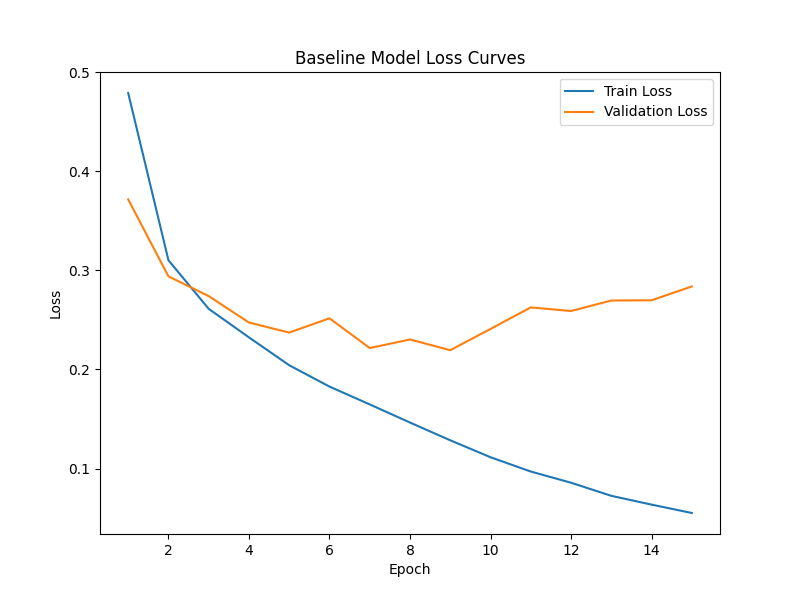
\includegraphics[width=\linewidth]{baseline_loss_curves.png}
			\caption{Baseline Model Loss Curves}
			\label{fig:baseline_loss}
		\end{subfigure}
		\hfill
		\begin{subfigure}{0.49\linewidth}
			\centering
			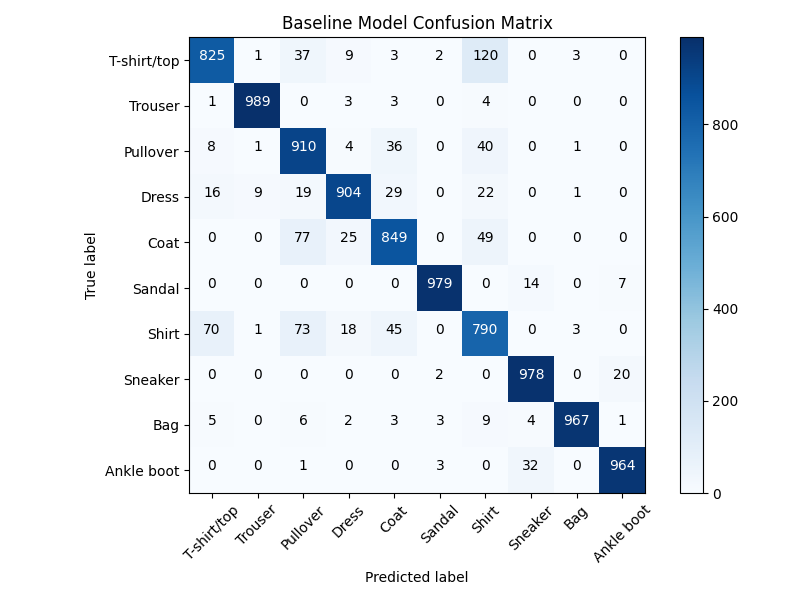
\includegraphics[width=\linewidth]{baseline_confusion_matrix.png}
			\caption{Baseline Model Confusion Matrix}
			\label{fig:baseline_conf_mat}
		\end{subfigure}
		\caption{Baseline Model: Loss Curves and Confusion Matrix}
		\label{fig:baseline_sidebyside}
	\end{figure}
	
	\subsection*{Improved CNN Model}
	
	In contrast, the improved model, enhanced with batch normalization and dropout ,achieves a test accuracy of 92.07\% on the held-out test set. As depicted in Figure \ref{fig:improved_loss}, the training and validation losses converge after approximately 10 epochs, indicating a more stable learning process and better generalization to unseen data. This convergence demonstrates that the model mitigates overfitting, likely due to the regularization effects of dropout and the stabilization provided by batch normalization.
	
	\begin{figure}[H]
		\centering
		\begin{subfigure}{0.49\linewidth}
			\centering
			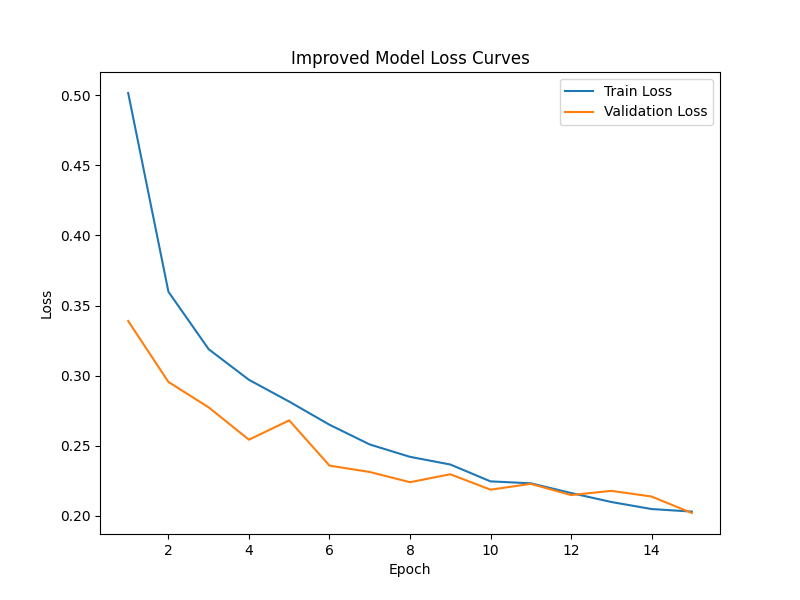
\includegraphics[width=\linewidth]{improved_loss_curves.png}
			\caption{Improved Model Loss Curves}
			\label{fig:improved_loss}
		\end{subfigure}
		\hfill
		\begin{subfigure}{0.49\linewidth}
			\centering
			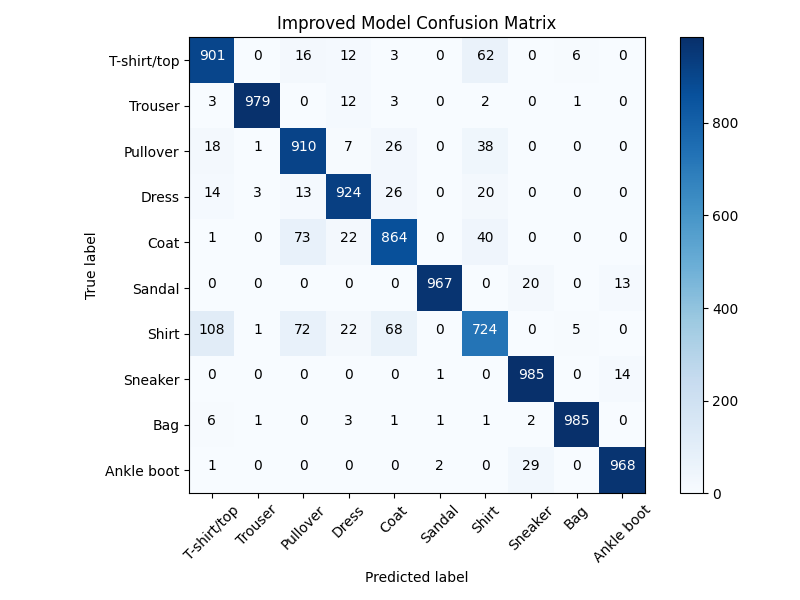
\includegraphics[width=\linewidth]{improved_confusion_matrix.png}
			\caption{Improved Model Confusion Matrix}
			\label{fig:improved_conf_mat}
		\end{subfigure}
		\caption{Improved Model: Loss Curves and Confusion Matrix}
		\label{fig:improved_sidebyside}
	\end{figure}
	
	\section{Ablation Studies}
	Two primary modifications were evaluated in the improved CNN model.
	\begin{enumerate}
		\item \textbf{Dropout Layers:} Their inclusion helped in reducing overfitting by randomly disabling parts of the network during training.
		\item \textbf{Batch Normalization:} This helped stabilize learning and allowed for faster convergence by normalizing the inputs to each layer.
	\end{enumerate}
	Comparing the two models, it is evident that the modifications led to:
	\begin{itemize}
		\item Model convergence between the training and validation losses, which suggests that the final model is less likely to overfit towards the training set.
		\item An improvement in test accuracy, increasing from 91.55\% on the base to 92.07\% on the improved model as evaluated on the held-out test set.
	\end{itemize}
	
	\section{Conclusion}
	This assignment implemented a CNN to classify images from the FashionMNIST dataset. Two models were compared: the baseline CNN and an improved version incorporating dropout and batch normalization. While both models performed well, the improved model demonstrated convergence between training and validation losses and achieved a higher test accuracy (92.07\% compared to 91.55\%) as evaluated on the held-out training set. These results suggest that regularization through dropout and stabilizing techniques like batch normalization can enhance model performance on image classification tasks.
	
	\section{Code Availability}
	The complete source code can be accessed at \url{https://github.com/echung32/ics635-cnn-fashion-mnist}.
	
\end{document}
